Keskitetyn tunnistautumisen lähtökohta on käyttäjän tunnistetietojen poistaminen web-palvelun hallinnasta. Käyttäjä ei syötä tunnistetietojaan missään vaiheessa web-palveluun, vaan tunnistautuminen tehdään keskitetyssä paikassa. Nykyisin mm. Facebook ja Google tarjoavat julkiset API-rajapinnat, joiden avulla web-palvelut voivat käyttää niitä tunnistautumiseen.

Kuvassa \ref{facebook_login} on kuvattu kirjautuminen Porkkanamafia-ryhmän WWW-sivulle käyttäen Facebookia. Käyttäjä klikkaa WWW-sivulla olevaa "Login with Facebook" -nappia, jonka jälkeen käyttäjän selaimeen avautuu Facebookin varmennusikkuna, jossa käyttäjää pyydetään varmentamaan kirjautuminen. Selaimen osoitekenttä osoittaa käyttäjälle, että kirjautuminen tapahtuu nimenomaan Facebook-sivulla (joka on varmennettu SSL-sertifikaatilla), joten käyttäjän Facebook-tunnistetiedot eivät päädy Porkkanamafian haltuun, vaan kirjautuminen hoidetaan suoraan Facebookiin.

Kirjautumisen jälkeen käyttäjälle luodaan rivi käyttäjätietokantaan, jossa on viittaus hänen Facebook-tunnukseen. Tämän jälkeen, kun käyttäjä palaa sivulle, ja kirjautuu jälleen Facebook-tunnuksilla, voidaan Facebookilta tullut käyttäjä yhdistää kannasta löytyvään vanhaan käyttäjään. Näin palvelu on ulkoistanut tunnistautumisen ulkopuoliselle taholle, eikä käyttäjän tarvitse muistaa uusia tunnistetietoja, vaan hän voi käyttää Facebook-kirjautumista jatkossa.

\begin{figure}[ht]
\centering
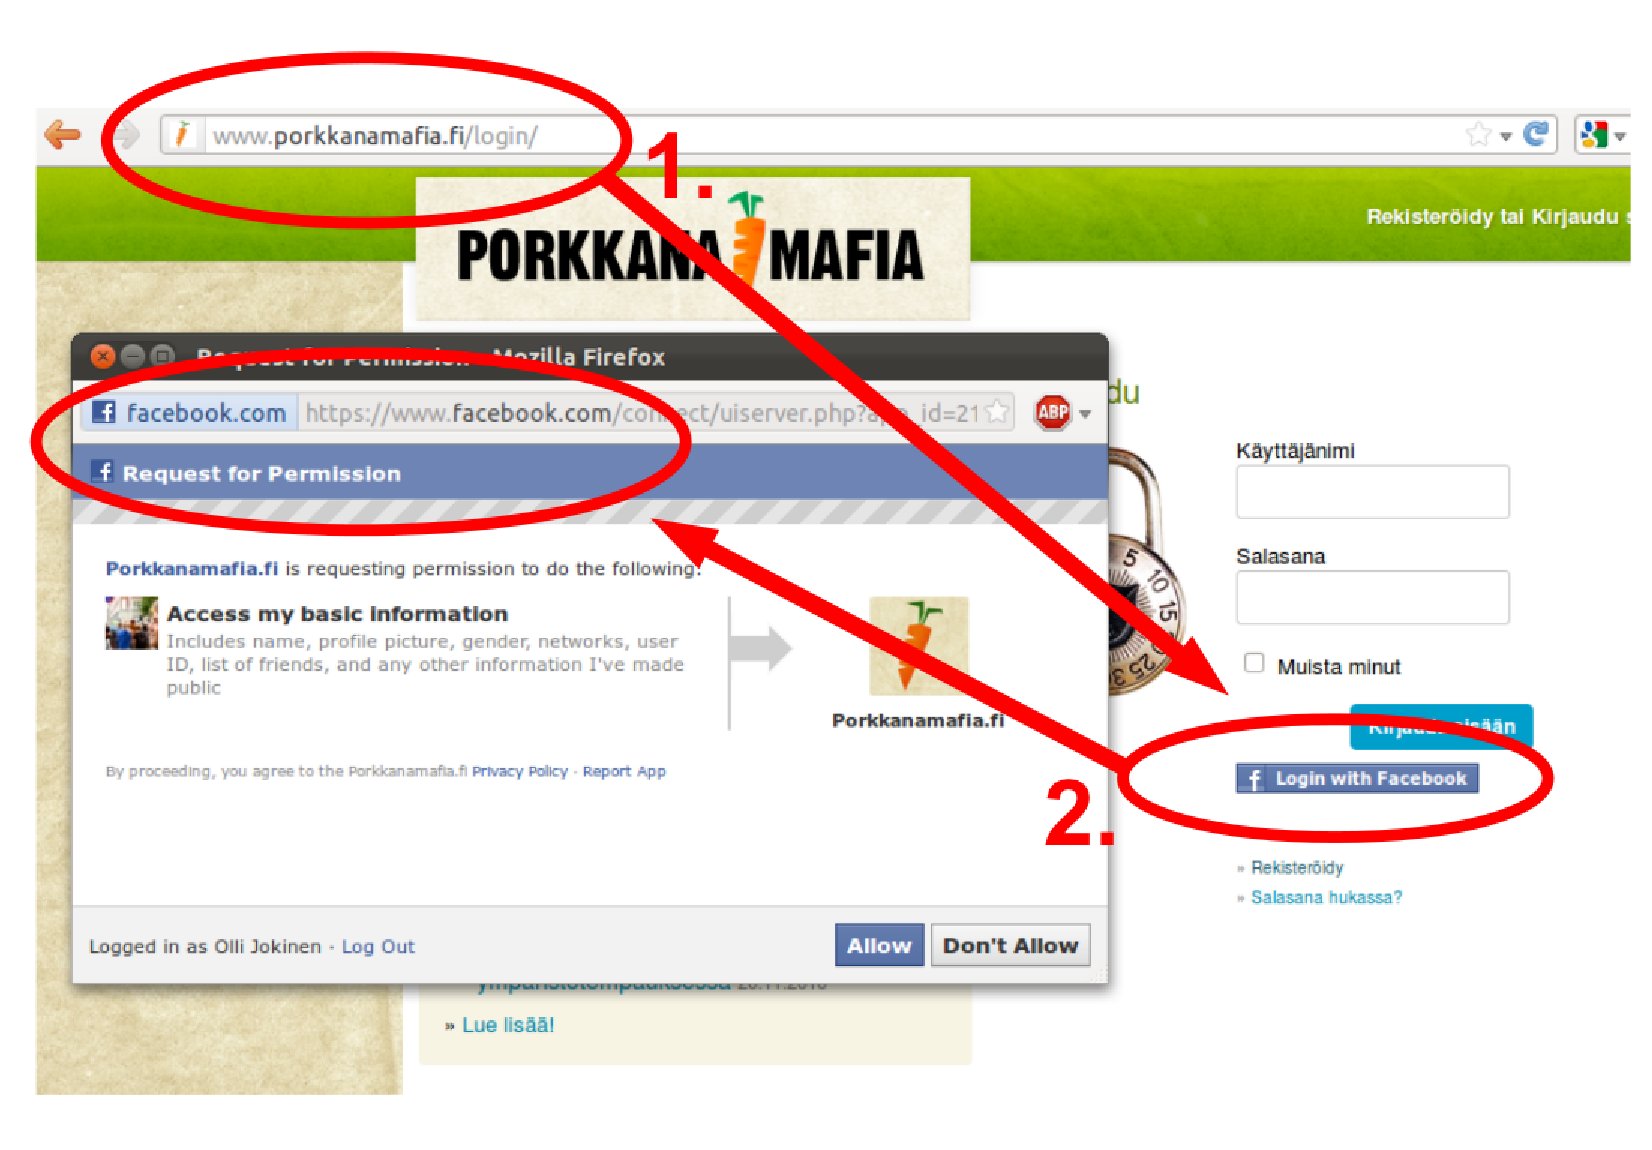
\includegraphics[width=\textwidth]{teknologiat/facebook.eps}
\caption{Käyttäjän kirjautuminen Facebook-tunnuksilla Porkkanamafian web-palveluun}%
\label{facebook_login}
\end{figure}

Samaa periaatetta voidaan käyttää myös organisaatioiden sisäisessä tunnistautumispalvelussa. Organisaation sisäiseen palvelusuuntautuneeseen arkkitehtuuriin toteutetaan erillinen web-palvelu, joka on yhteydessä olemassa olevaan käyttäjätietokantaan (esim. LDAP), ja tarjoaa Facebookia vastaavan tunnistautumisen.

Keskitetty tunnistautumispalvelun periaate on kuvattu kuvassa \ref{composition}, jossa on neljä palveluun kuuluvaa komponenttia. Ensimmäiseksi käyttäjä menee WWW-selaimen avulla web-palveluun, joka pyytää tunnistautumista erillisessä tunnistautumispalvelussa. Käyttäjän selain ohjataan tunnistautumispalvelun sivulle, joka on yhteydessä organisaation käyttäjähallintaan. Jos käyttäjähallinnasta löytyy käyttäjän syöttämät tunnistetiedot, palautetaan käyttäjälle valtuutusavain, jonka käyttäjä lähettää takaisin web-palvelulle. Tämän jälkeen web-palvelu varmistaa tunnistautumispalvelulta valtuutusavaimen oikeellisuuden ja tunnistautumispalvelu palauttaa käyttäjän tiedot web-palvelulle.

\begin{figure}[ht]
\centering
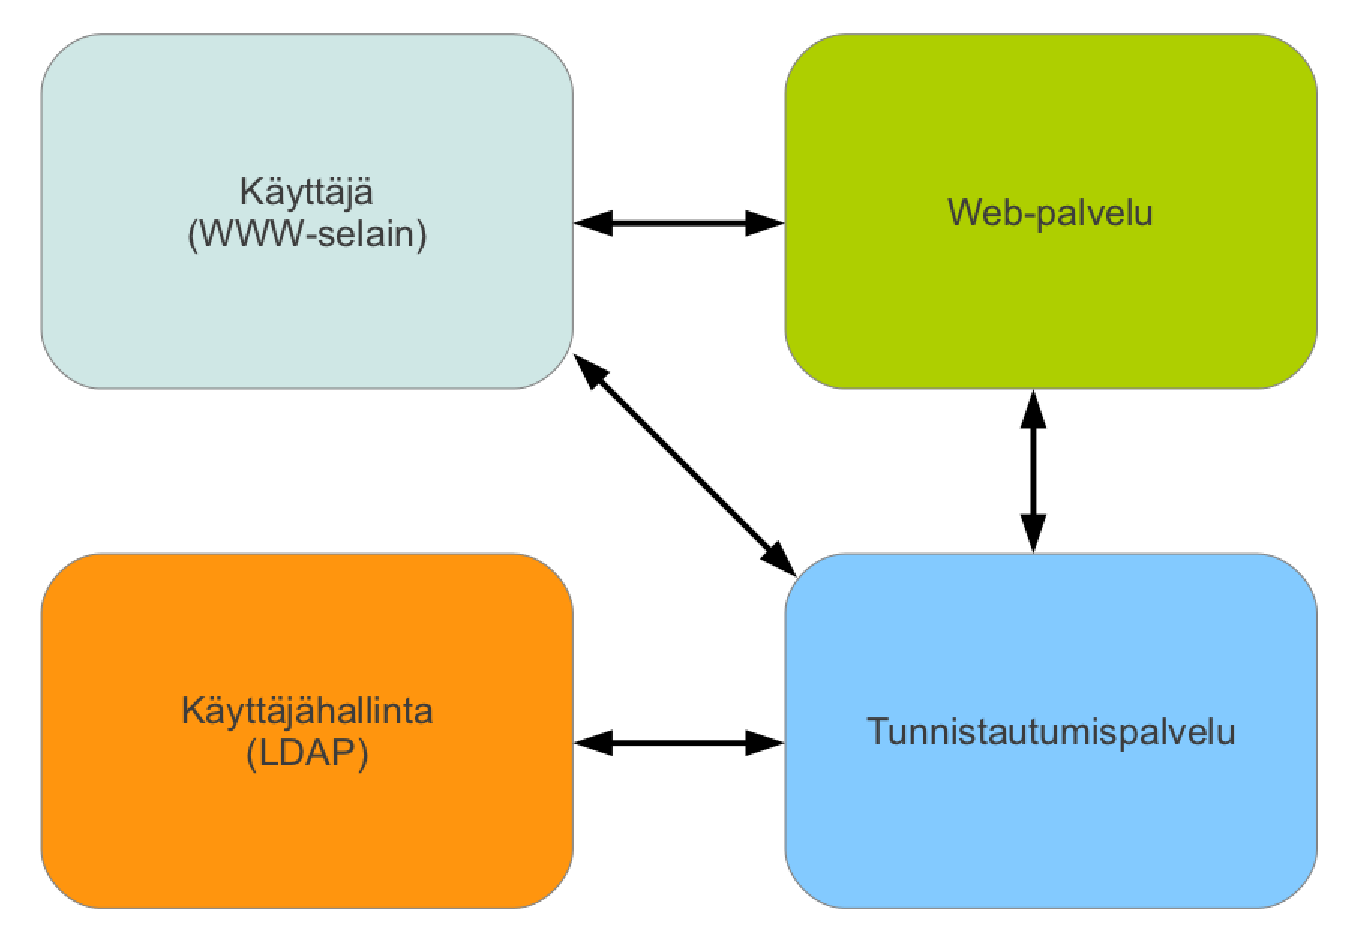
\includegraphics[width=\textwidth]{teknologiat/composition.eps}
\caption{Keskitetyn tunnistautumisen periaatteet}%
\label{composition}
\end{figure}
